% --- Ha \& Schmidhuber (2018): V--M--C architecture ---
\begin{frame}{World Model Overview}
    \centering
    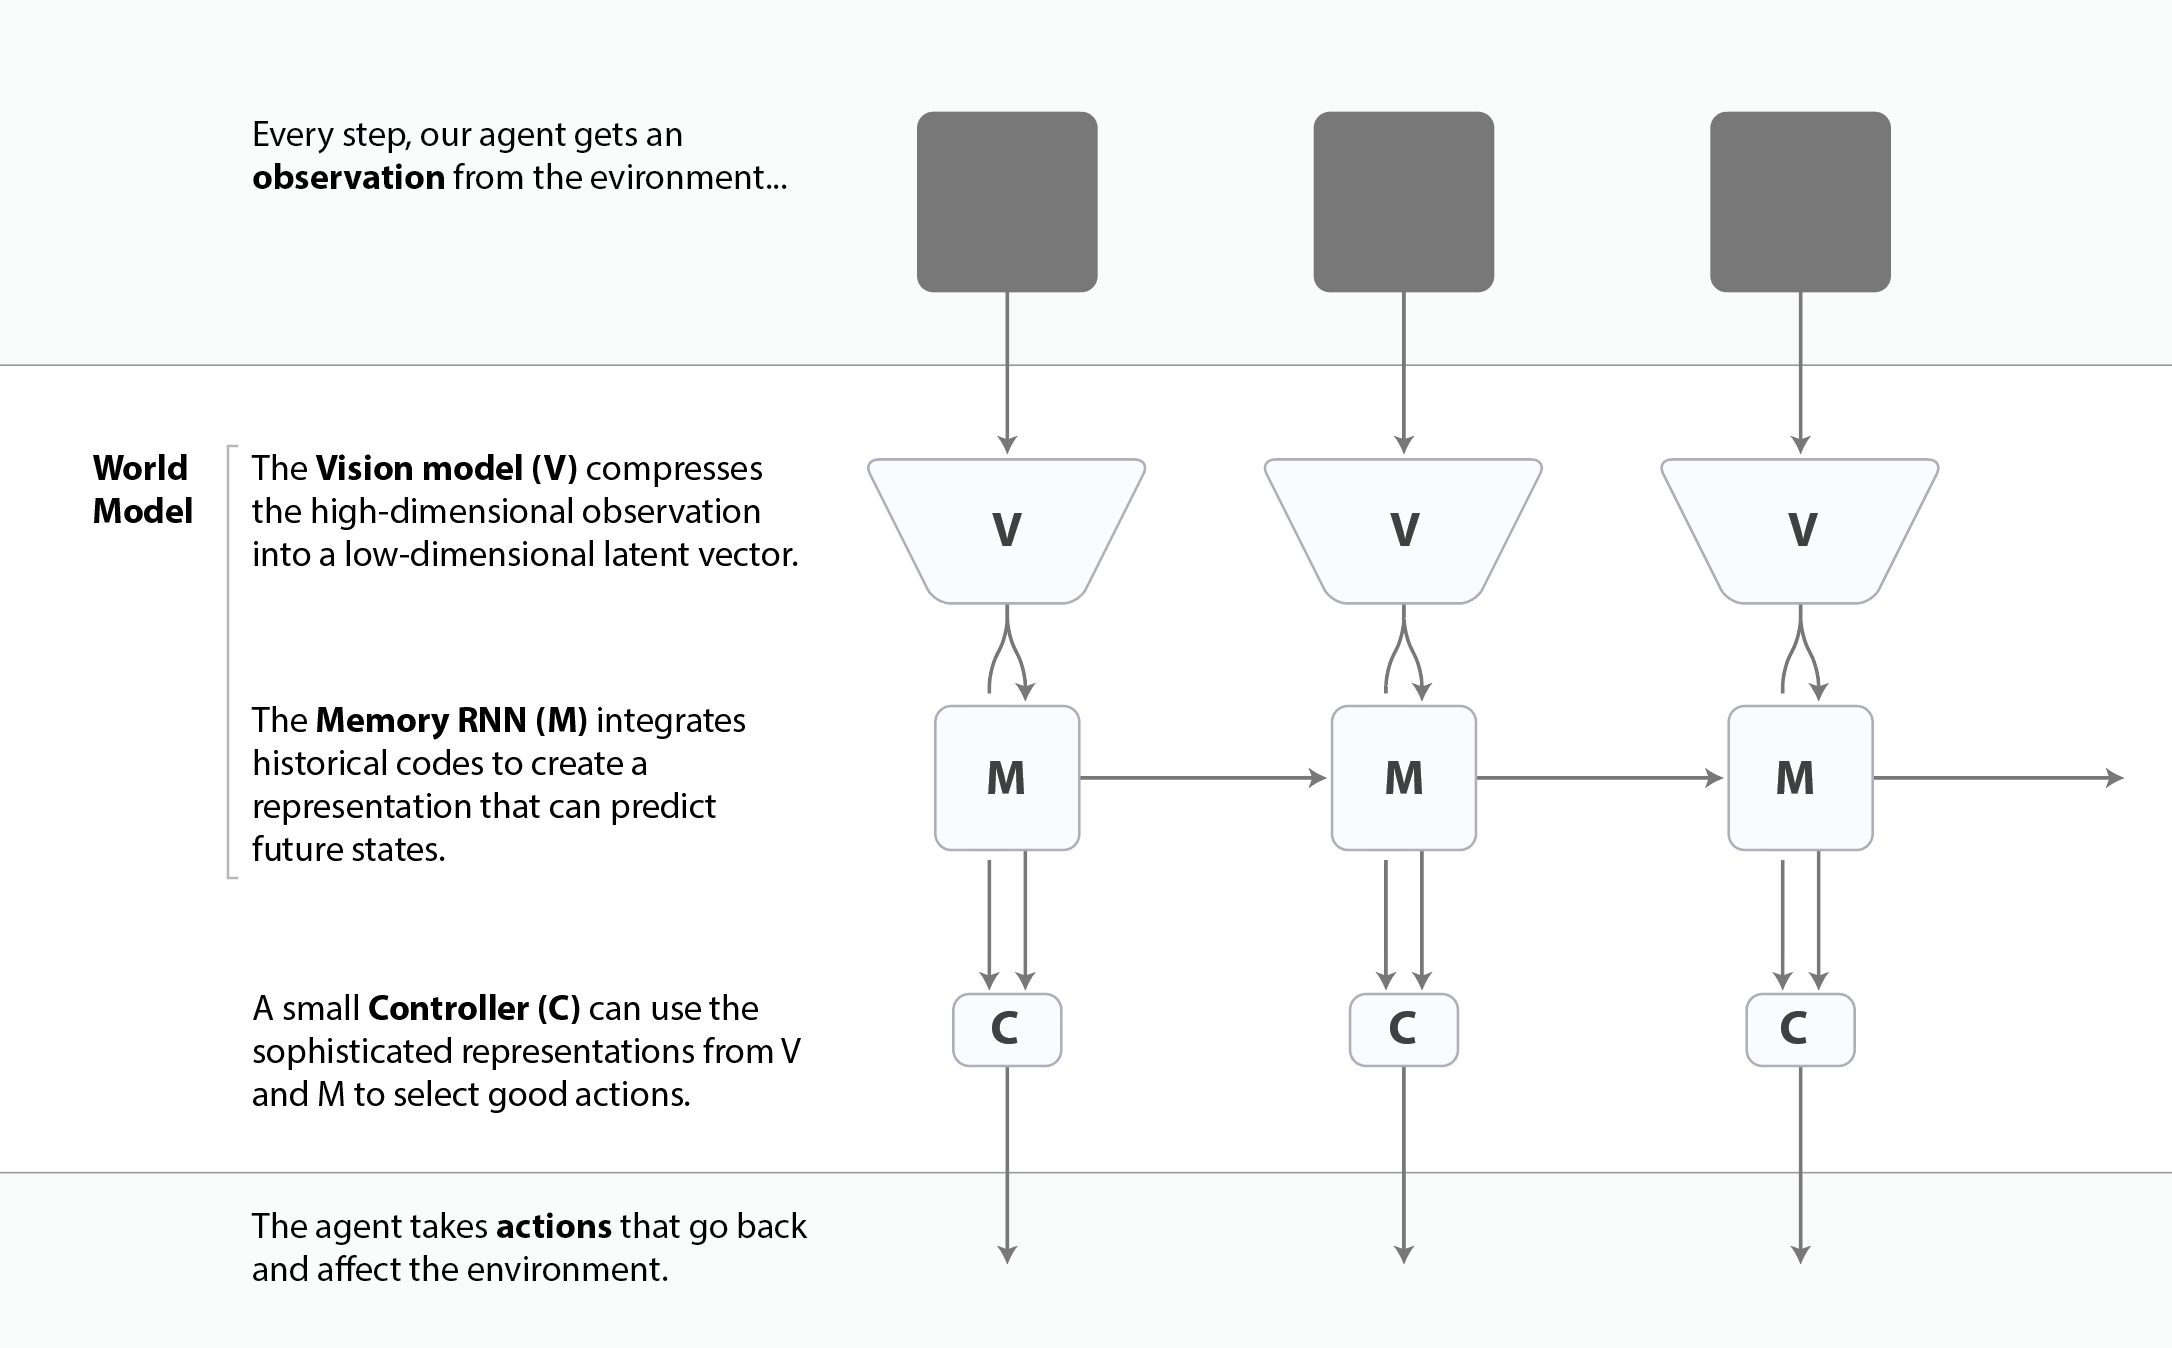
\includegraphics[width=0.95\linewidth,height=0.88\textheight,keepaspectratio]{assets/New-Lecture_World_Models/worldmodels_githubio_rollout_schematic.png}\\[0.15em]
    {\scriptsize World model overview.\\
    \textit{Source: Ha \& Schmidhuber, 2018}}
\end{frame}

\begin{frame}{Vision module: variational autoencoder (V)}
  \begin{columns}[T,onlytextwidth]
    \column{0.44\textwidth}
    \begin{itemize}\itemsep0.26em
      \item[\textcolor{red}{$\blacktriangleright$}] \textbf{Goal:} learn an abstract, compressed representation of each observed input frame.
      \item[\textcolor{red}{$\blacktriangleright$}] \textbf{VAE:} first stage of a two-stage sequence model---similar in spirit to modern tokenizers, but trained with classic VAE objective.
    \end{itemize}
    \column{0.54\textwidth}
    \centering
    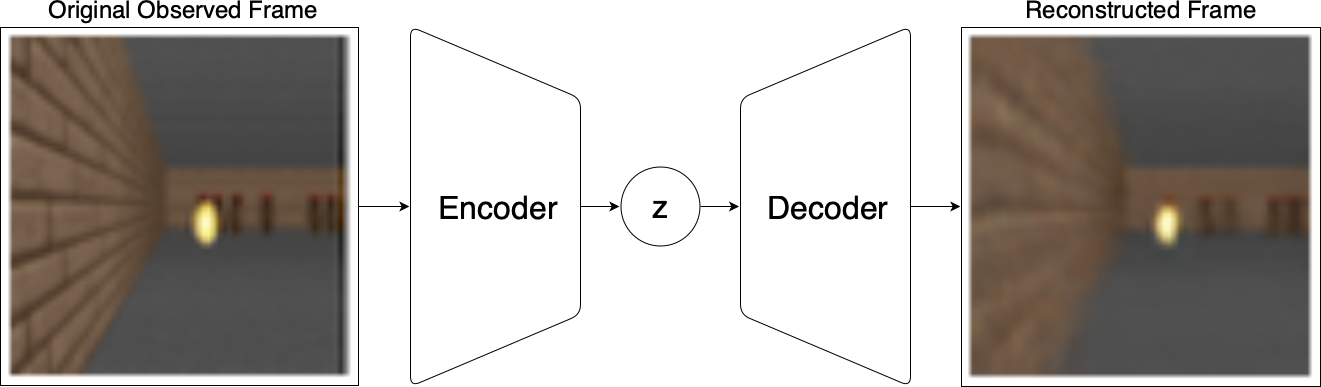
\includegraphics[width=0.95\linewidth,height=0.88\textheight,keepaspectratio]{assets/New-Lecture_World_Models/worldmodels_githubio_vae.png}\\[0.15em]
    {\scriptsize VAE diagram.\\
    \textit{Source: Ha \& Schmidhuber, 2018}}
  \end{columns}
\end{frame}

\begin{frame}{Memory module: Predict the future}
  \begin{columns}[T,onlytextwidth]
    \column{0.42\textwidth}
    \begin{itemize}\itemsep0.26em
      \item[\textcolor{red}{$\blacktriangleright$}] Model $p(z_{t+1} \mid z_t, a_t, h_t)$ where $z_t$ is the latent state at time $t$, $a_t$ is the action at time $t$, and $h_t$ is the hidden state at time $t$.
      \item[\textcolor{red}{$\blacktriangleright$}] adjust a temperature parameter $\tau$ to control model uncertainty
    \end{itemize}
    \column{0.56\textwidth}
    \centering
    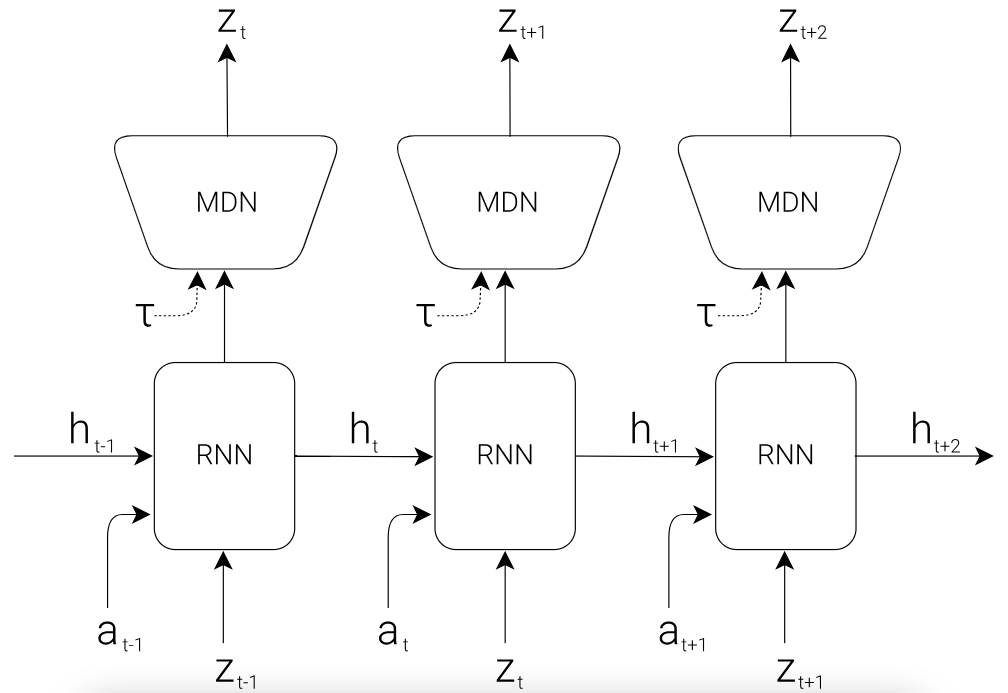
\includegraphics[width=0.95\linewidth,height=0.76\textheight,keepaspectratio]{assets/New-Lecture_World_Models/mdn_rnn_new.png}\\[0.15em]
    {\scriptsize MDN-RNN architecture.\\
    \textit{Source: Ha \& Schmidhuber, 2018}}
  \end{columns}
\end{frame}


\begin{frame}{Controller module: decision-making (C)}
    \begin{itemize}\itemsep0.26em
      \item[\textcolor{red}{$\blacktriangleright$}] The \textbf{Controller (C)} selects actions to maximize expected cumulative reward during agent rollout.
      \item[\textcolor{red}{$\blacktriangleright$}] Designed to be as simple and small as possible; trained \textbf{separately} from the Vision (V) and Memory (M) modules.
      \item[\textcolor{red}{$\blacktriangleright$}] Most agent complexity is thus concentrated in the world model (V and M).
      \item[\textcolor{red}{$\blacktriangleright$}] C is a \textbf{single-layer linear} model that maps the latent vector $z_t$ and RNN hidden state $h_t$ directly to the action $a_t$ at each time step:
    \end{itemize}
    \vspace{0.7em}
    {\small
    \[
      a_t = W_c [z_t; h_t] + b_c
    \]
    }
    \begin{itemize}\itemsep0.15em
      \item[\textcolor{red}{$\blacktriangleright$}] Here, $W_c$ and $b_c$ are the weight matrix and bias; $[z_t; h_t]$ is the concatenated latent and memory state.
      \item[\textcolor{red}{$\blacktriangleright$}] Output vector $a_t$ is the action taken by the agent.
    \end{itemize}
    % Optionally: say evolved with CMA-ES, not trained end-to-end.
\end{frame}

\begin{frame}{World model: Putting Everything Together}
  \centering
  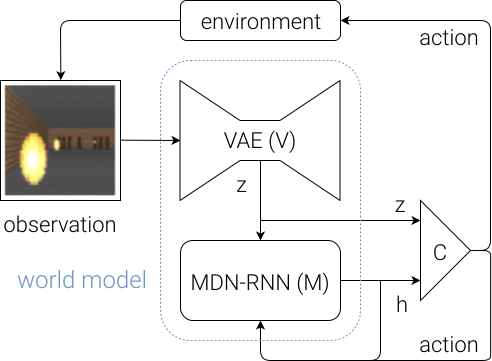
\includegraphics[width=\linewidth,height=0.88\textheight,keepaspectratio]{assets/New-Lecture_World_Models/world_model_schematic_downloads.png}\\[0.28em]
  {\scriptsize Agent-environment flow (observation $\rightarrow$ $z_t$, RNN state $h_t$, action $a_t$, next step).\\
  \textit{Source: Ha \& Schmidhuber, 2018}}
\end{frame}
\begin{frame}{Takeaways}
  \begin{itemize}
    \item \textbf{Separation of concerns:} perception (VAE), dynamics (RNN), decision (controller)---easy to prototype but may \textbf{not} share gradients end-to-end through the full agent loop at scale.
    \item \textbf{Stochastic latents} matter: the world is multi-modal; Gaussian or MDN heads encode ``many possible futures''.
    \item Next step (PlaNet, Dreamer): unify training with \textbf{RSSM}-style latent dynamics and \textbf{model-based RL} losses.
  \end{itemize}
\end{frame}
